\documentclass{article}

\usepackage{graphicx} % Required for inserting images
\usepackage{hyperref}
\usepackage[
    backend = biber,
    style = abnt,
    ]{biblatex}
\addbibresource{bibliografia.bib}
\usepackage[shortlabels]{enumitem}
\usepackage[brazilian]{babel}

\title{%
  Direito Internacional Público \\
  \Large Notas de Aula 5\\
  \Large O Estado: território\\
  }
\author{Luccas Gissoni}
\date{8 de outubro de 2024}

\begin{document}

\maketitle
\tableofcontents

\section{Introdução}

O Estado, persolaidade de direito internacional público, ostenta três elementos:

\begin{enumerate}
    \item \textbf{Base territorial}
    \item \textbf{Comunidade humana} estabelecida nessa área
    \item Forma de \textbf{governo} não subordinada a qualquer autoridade exterior
\end{enumerate}

Nesta aula trataremos do primeiro elemento, isto é, do \textbf{território}.

\begin{quote}
    Variam grandemente, de um Estado a outro, as dimensões territoriais e demográficas, assim como variam as formas de organização política. Acresce que, em circunstâncias excepcionais e transitórias, pode faltar ao Estado o elemento governo — tal é o que sucede nos períodos anárquicos —, e pode faltar-lhe até mesmo a disponibilidade efetiva de seu território, ou o efetivo controle dessa base por seu governo legítimo. O elemento humano é, em verdade, o único que se supõe imune a qualquer eclipse, e cuja existência ininterrupta responde, mais que a do próprio elemento territorial, pelo princípio da continuidade do Estado — de que falaremos mais tarde, no estudo da sucessão de Estados \cite[p.~72]{rezek_direito_2024}.
\end{quote}

\section{Jurisdição ou competência}

\begin{quote}
    Sobre seu território o Estado exerce jurisdição (termo preferido em doutrina anglo-saxônica), o que vale dizer que detém uma série de competências para atuar com autoridade (expressão mais ao gosto dos autores da escola francesa). O território de que falamos é a área terrestre do Estado, somada àqueles espaços hídricos de topografia puramente interna, como os rios e lagos que se circunscrevem no inte­rior dessa área sólida. Sobre o território assim entendido, o Estado soberano tem jurisdição \textbf{geral} e \textbf{exclusiva} \cite[p.~72]{rezek_direito_2024}.
\end{quote}

\subsection{Generalidade}

\begin{quote}
    A generalidade da jurisdição significa que o Estado exerce no seu domínio territorial todas as competências de ordem legis­lativa, administrativa e jurisdicional \textbf{geral} e \textbf{exclusiva} \cite[p.~72]{rezek_direito_2024}.
\end{quote}

\subsection{Exclusividade}

\begin{quote}
    A exclusividade significa que, no exercício de tais competências, o Estado local não enfrenta a concorrência de qualquer outra soberania. Só ele pode, assim, tomar medidas restritivas contra pessoas, detentor que é do monopólio do uso legítimo da força pública \textbf{geral} e \textbf{exclusiva} \cite[p.~72]{rezek_direito_2024}.
\end{quote}

\section{Aquisição e perda de território}

\subsection{Descoberta - ocupação: \textit{terra nullius}}

Aquisição por descoberta de determinado território seguida de ocupação efetiva ou presumida. O território objeto desse tipo de aquisição é a \textit{terra nullius}, ou terra de ninguém.

Associado à descoberta da \textit{terra nullius} está o princípio da \textit{contiguidade}: ``a pretensão ocupacionista do descobridor avança pelo território adentro até quando possível — em geral, até encontrar a resistência de uma pretensão alheia congênere" \cite[p.~73]{rezek_direito_2024}

\paragraph{Controvérsia de Valladolid (1550-1551)}
\begin{itemize}
    \item \textbf{Ginés de Sepúlveda}: é justa a guerra e escravização dos índios porque estes são seres inferiores
    \item \textbf{Bartolomé de Las Casas}: refuta a pretensão de superioridade da cultura ocidental, da qual se deduz a barbárie das culturas indígenas
\end{itemize}

\paragraph{Felipe Guamán Poma de Ayala (1534-1615)}Espanhóis pregam os mandamentos do Evangelho, mas agem de forma contraditória

\paragraph{Exercício}
Quem é o autor dos seguintes textos?
\begin{enumerate}
    \item ``E se rejeitarem tal império, pode ser imposto a eles por meio de armas, e tal guerra será justa de acordo com a lei natural declara isso [...] Em suma: é justo, conveniente e de acordo com a lei natural que os homens justos, inteligentes, virtuosos e humanos dominem todos os que não possuem essas qualidades”
    \item ``Conceda-se que os Índios do tempo dos Incas idolatraram como gentios e adoravam ao sol, pai do Inca e a lua, sua mãe, e as estrelas seus irmãos [...] Com tudo isso eles guardaram os mandamentos e as boas obras de misericórdia de Deus neste reino, o que não é mantido pelos cristãos”
    \item ``Eles [os índios] não são homens? Eles não têm almas racionais? Você não está
forçados a amá-los como a si mesmos? [...] Como você está com tanto
profundidade do sono tão letárgico?"
\end{enumerate}

\subsection{Conquista}

Aquisição do território como resultado do emprego da força unilateral ou do triumfo em campo de batalha.\\

\href{https://youtu.be/UY9P0QSxlnI}{Vídeo: como o mapa da Europa tem mudado ao longo de 2400 anos}

\begin{quote}
    Hoje, entretanto, não seria possível admitir a conquista como meio de aquisição territorial, desde que proscrito o recurso às armas pelo direito das gentes. Assim, Israel não pretendeu ter-se investido no domínio dos territórios palestinos cujo controle resultou de seu êxito na guerra de 1967 e em conflitos posteriores: a necessidade de fronteiras seguras foi seu argumento para a retenção dessas áreas, até que o abrandamento das tensões políticas permitisse negociação construtiva com países vizinhos e com a liderança palestina \cite[p.~73; cf. figuras \ref{fig:guerra_6_dias} e \ref{fig:territorios_palestinos_ocupados}]{rezek_direito_2024}.
\end{quote}

\begin{figure}
    \centering
    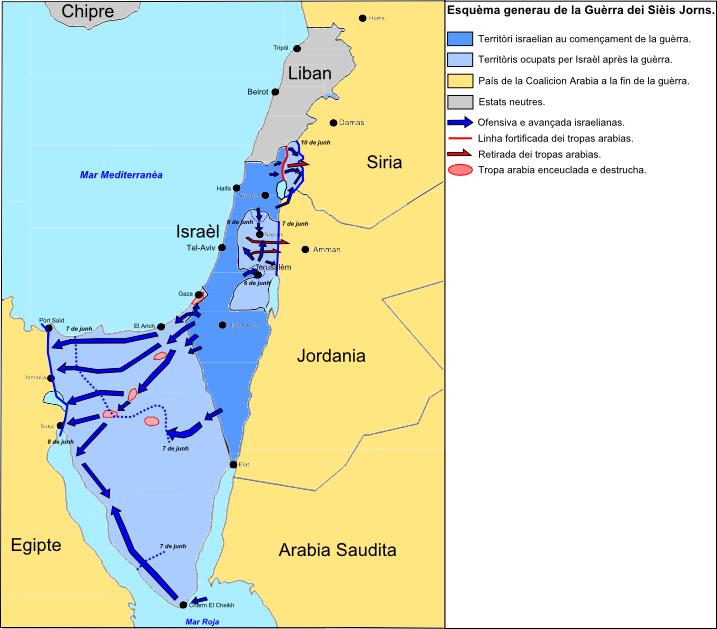
\includegraphics[width=0.75\linewidth]{guerra_6_dias.png}
    \caption{Território ocupado por Israel na Guerra dos Seis Dias (1967).}
    \label{fig:guerra_6_dias}
\end{figure}

\begin{figure}
    \centering
    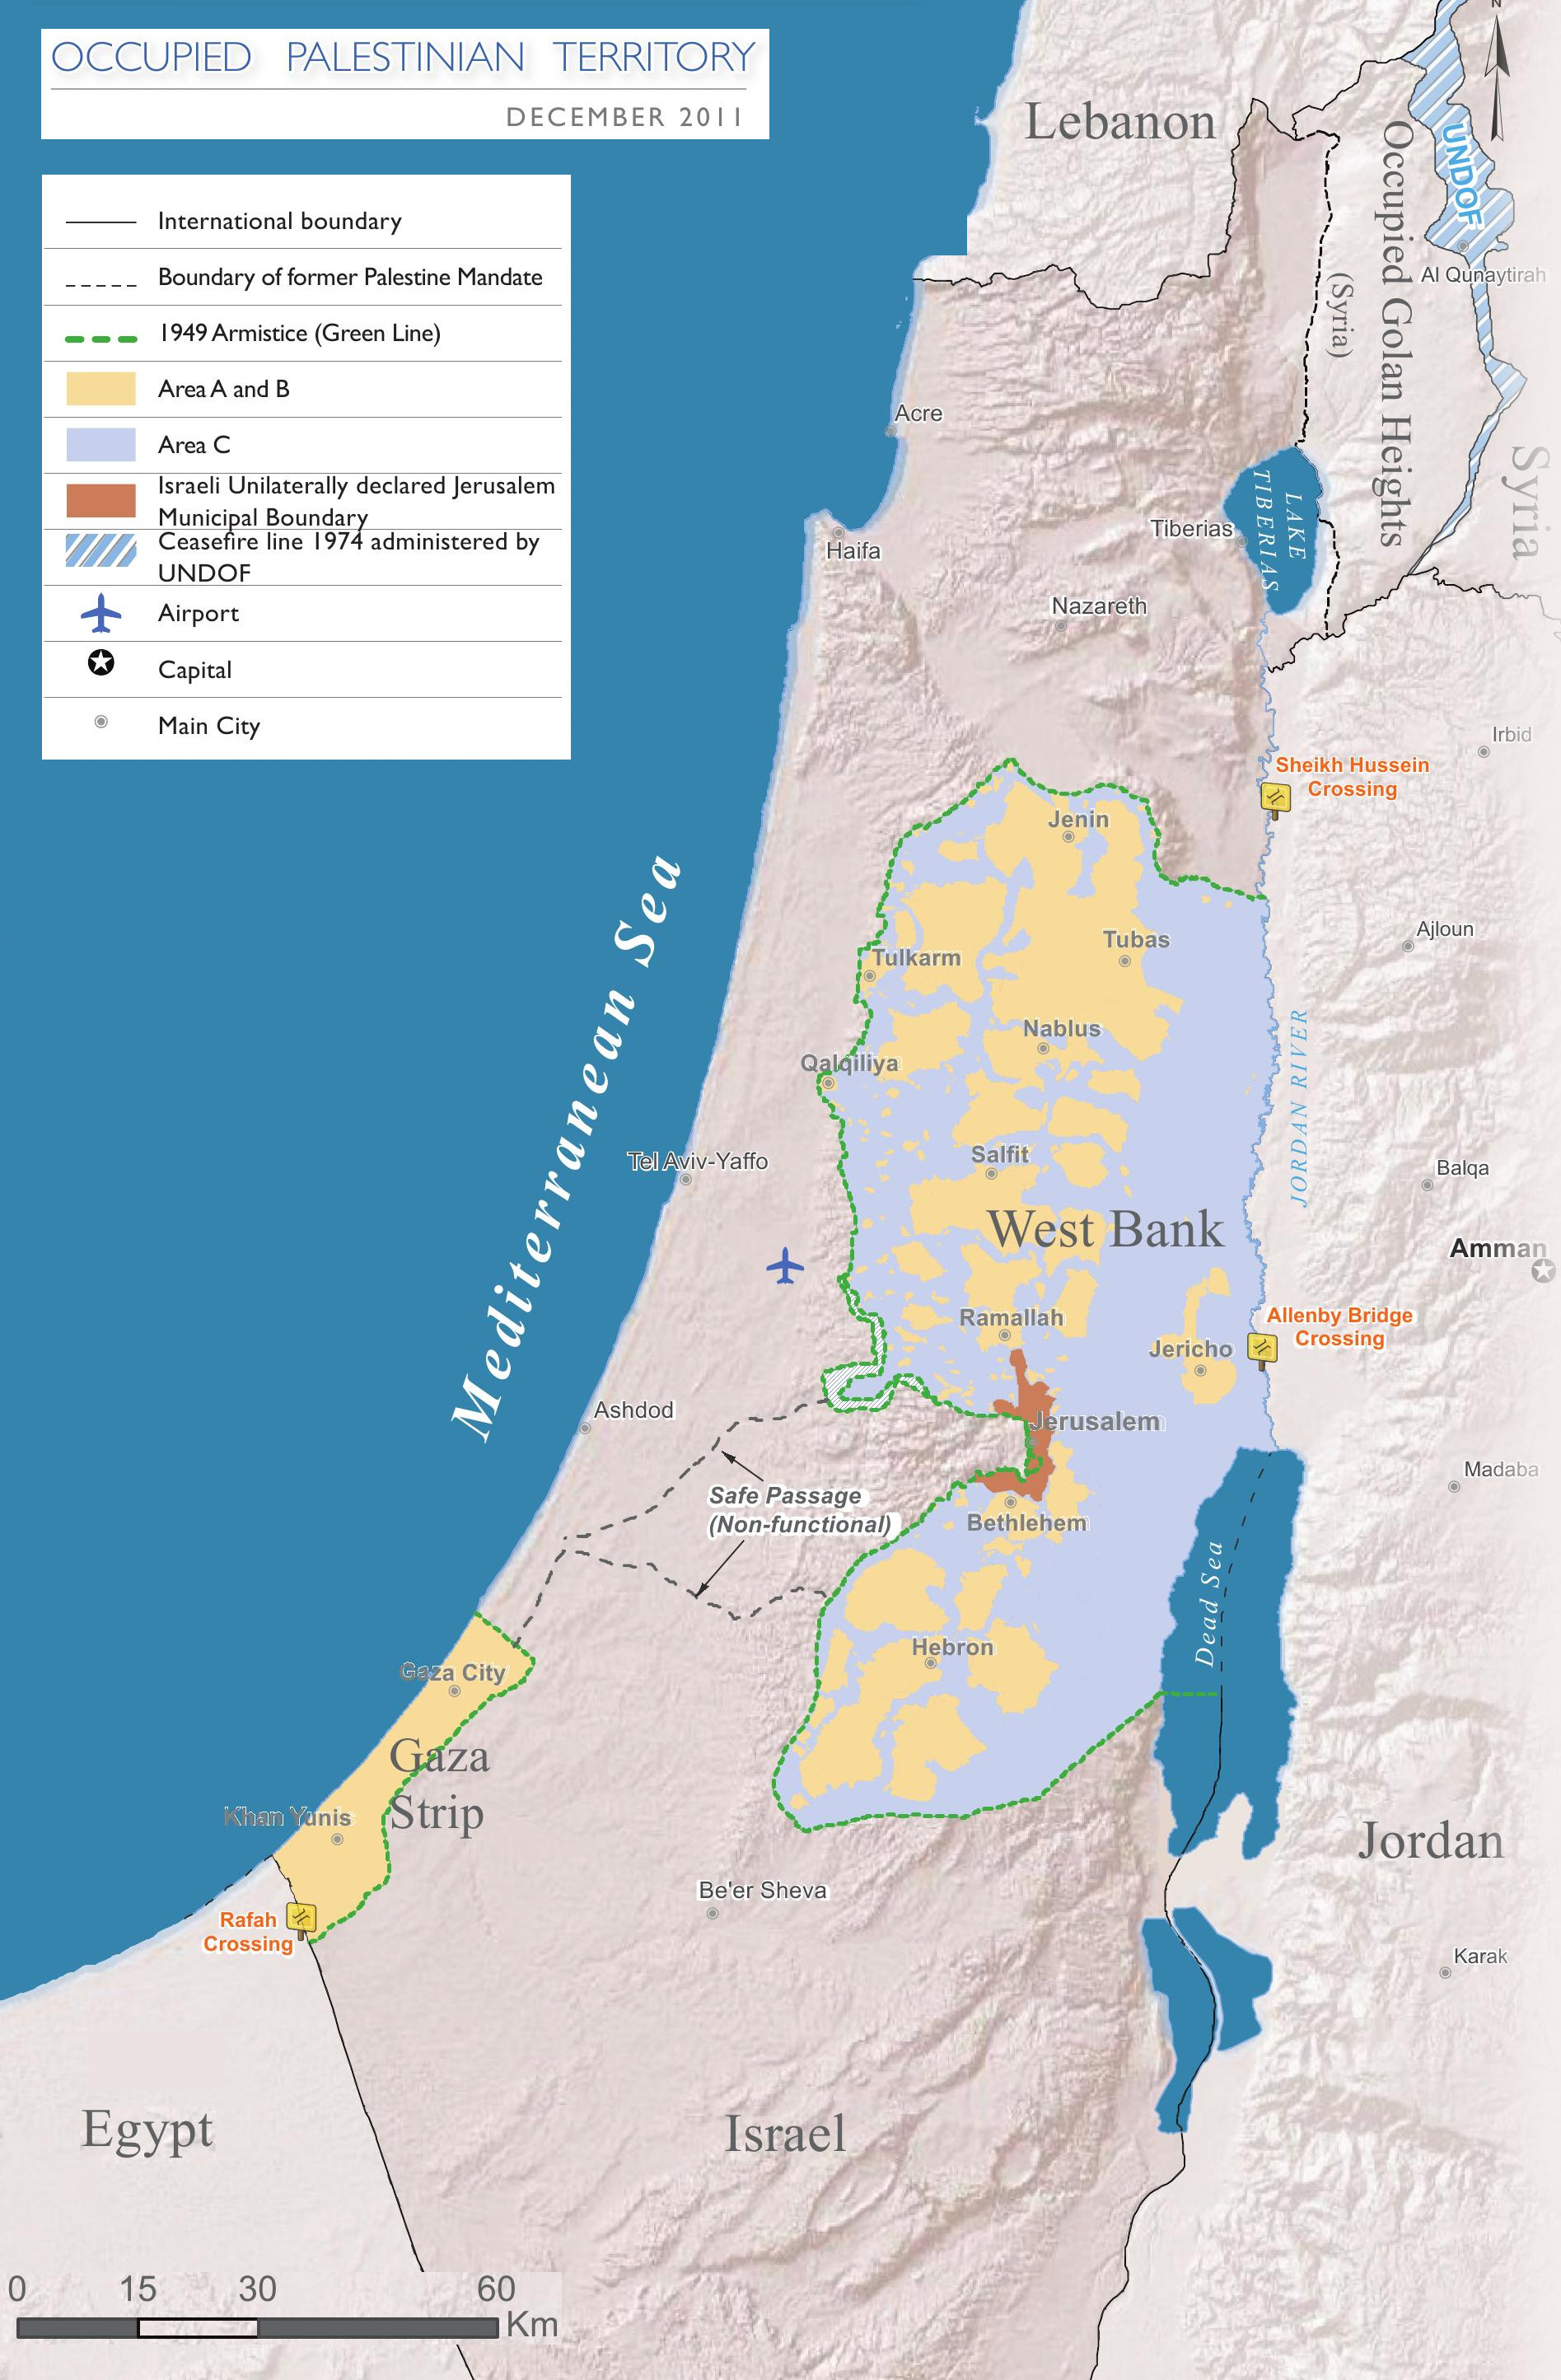
\includegraphics[width=0.75\linewidth]{territorios_palestinos_ocupados.jpg}
    \caption{Território palestino ocupado por Israel (2011).}
    \label{fig:territorios_palestinos_ocupados}
\end{figure}

\subsection{Cessão onerosa}

Aquisição do território por meio da compra e venda ou da permuta.

\begin{quote}
    Os Estados Unidos da América compraram a Louisiana da França em 1803, por 60 milhões de francos, e o Alasca da Rússia em 1867, por 7,2 milhões de dólares. O Brasil adquiriu o Acre da Bolívia em 1903, mediante o pagamento de 2 milhões de libras esterlinas e a prestação de determinados serviços \cite[p.~73]{rezek_direito_2024}.
\end{quote}

\subsubsection{Cessão gratuita}

\begin{quote}
    A história registra casos de cessão gratuita — um evidente eufemismo, visto que mal se compreende por que um Estado faria a doação de parte do seu território, a menos que não tivesse escolha. A cessão gratuita foi um ornamento típico dos tratados de paz, aqueles em que, finda a guerra, defrontavam-se na mesa de negociação vencedores e vencidos, estes à mercê daqueles.
    \\Mediante cessão gratuita a França, derrotada na guerra bilateral, cedeu a Alsácia-Lorena à Alemanha em 1871. Quase meio século mais tarde, ao termo da primeira grande guerra, a Alemanha está vencida e a França perfila entre os vitoriosos: nova cessão gratuita, em sentido inverso, restitui a Alsácia-Lorena à soberania francesa, consignando-se no texto do Tratado de Versalhes (1919) \cite[p.~73]{rezek_direito_2024}.
\end{quote}

\subsubsection{Decisão de organizações internacionais}

\begin{quote}
    A atribuição de território por decisão política de uma organização internacional ocorreu no âmbito da ONU em 1947, a propósito da partilha da Palestina, e de novo em 1950 quanto às ex-colônias italianas na África. O órgão judiciário da ONU, qual seja a Corte da Haia, não atribui território: limita-se a dizer, à luz do direito aplicável, a quem certa área pertence, ou como os conten­dores deverão proceder para a correta partilha da região controvertida (casos do templo de Preah-Vihear, Camboja-Tailândia, 1962; do Camerum setentrional, Camerum-Reino Unido, 1963; da plataforma continental do mar do Norte, Dinamarca-Países Baixos-Alemanha, 1969; da ilha Kasikili-Sedudu, Botsuana-Namíbia, 1999; da delimitação marítima e terrestre Catar-Barém, 2001)  \cite[p.~73]{rezek_direito_2024}.
\end{quote}

\section{Delimitação territorial}

A noção da fronteira é produto da evolução histórica dos acontecimentos. Uma vez obtida essa noção, a fronteira normalmente é delimitada por um tratado bilateral entre os Estados vizinhos que pretendem atribuir a ela o exato traçado.

\subsection{\textit{Uti possidetis}}

\begin{quote}
    \textit{Uti possidetis ita possideatis} é mais um daqueles princípios de direito que evocam a lei física da inércia: como possuís, continuareis possuindo. Largamente empregado desde o início do século XIX na América hispânica, o princípio significava a conservação, pelas nações latino-americanas independentes, das fronteiras coloniais, ou seja, daquele traçado que já as separava enquanto províncias coloniais da Espanha. A isso deu-se o nome de \textit{uti possidetis juris} a partir do momento em que a América portuguesa, pouco interessada na cartografia do império colonial espanhol e nas bulas papais, privilegiou a ocupação efetiva das terras do novo continente e fez valer para si uma variante do princípio: o \textit{uti possidetis de facto}. A essa concepção brasileira do \textit{uti possidetis} dá-se hoje com frequência em doutrina, e sobretudo na jurisprudência da Corte da Haia, o nome de \textit{efetividades}, ou consideração do efetivo exercício da soberania sobre determinada área territorial. O \textit{uti possidetis juris}, o das repúblicas hispano-americanas, teria amplo emprego no continente africano ao longo do processo de descolonização, na segunda metade do século XX \cite[p.~74]{rezek_direito_2024}.
\end{quote}  

\subsection{Linhas artificiais x naturais}

\subsubsection{Linhas artificiais}

\begin{quote}
    No trabalho de delimitação, os Estados vizinhos tanto podem optar por linhas limítrofes artificiais quanto naturais. As primeiras são as linhas geodésicas (os paralelos e os meridianos), ou qualquer arranjo ou combinação que se imagine à base delas para o estabelecimento, por exemplo, de diagonais. O limite entre o Canadá e os Estados Unidos da América é, em grande parte, constituído por um paralelo. O mapa político da África revela, por sua vez, largo uso das linhas geodésicas para o traçado dos limites interestatais. O emprego de limites artificiais foi, contudo, pouco expressivo na Europa, na Ásia e na América Latina. \cite[p.~74]{rezek_direito_2024}.
\end{quote}

\subsubsection{Linhas naturais}

\begin{quote}
    Os limites naturais de generalizado prestígio são rios e cordilheiras. No caso destas, a exata linha limítrofe pode correr ao longo da base da cadeia montanhosa, em um de seus dois flancos, de modo que toda a cordilheira pertença a um só dos Estados confrontantes. É mais comum a opção pela linha das cumeeiras (uma linha quebrada, ligando pontos de altitude expressiva) ou pelo divortium aquarum — a linha onde se repartem as águas da chuva, escorrendo por uma ou outra das vertentes da cordilheira. Este último critério predomina na fronteira argentino-chilena dos Andes, bem assim nas divisas montanhosas do Brasil com a Venezuela, a Colômbia e o Peru.
    \\No caso dos rios, é compreensível que se evite lançar a linha limítrofe em uma de suas margens, consagrando o total domínio do curso d’água por um só dos Estados ribeirinhos. Preferem-se dois sistemas: o da linha de equidistância das margens (que passa pela superfície do rio, estando sempre no ponto central de sua largura), e o do talvegue ou linha de maior profundidade (que toma em consideração o leito do rio, e passa por suas estrias mais profundas). O talvegue é de uso mais frequente nos rios navegáveis: foi ele o critério limítrofe escolhido por Argentina e Brasil para os rios Uruguai e Iguaçu, por Brasil e Peru para o rio Purus, por Brasil e Colômbia para os rios Iquiare e Taraíra. A linha da equidistância foi preferida por Bolívia e Brasil a propósito dos rios Guaporé, Mamoré e Madeira \cite[p.~74]{rezek_direito_2024}.
\end{quote}

\printbibliography

\end{document}